\documentclass[tikz,border=5pt]{standalone}
\usepackage{amsmath}
\usepackage{pgfplots}
\pgfplotsset{compat=1.18}

\definecolor{corba}{HTML}{365FB3}
\definecolor{punt}{HTML}{B91C1C}
\definecolor{assimptota}{HTML}{6B7280}

\begin{document}
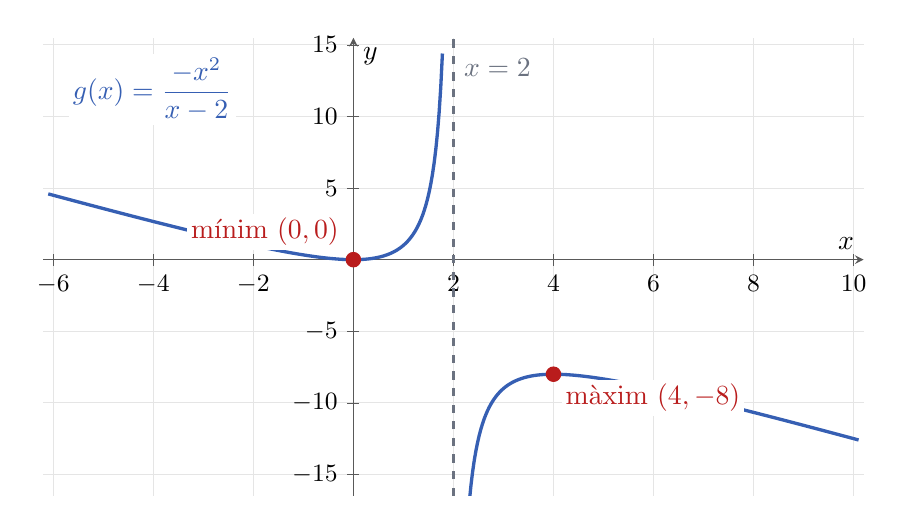
\begin{tikzpicture}
  \begin{axis}[
    width=12cm,
    height=7.4cm,
    axis lines=middle,
    xmin=-6.2,
    xmax=10.2,
    ymin=-16.5,
    ymax=15.5,
    xlabel={$x$},
    ylabel={$y$},
    xtick={-6,-4,-2,0,2,4,6,8,10},
    ytick={-15,-10,-5,0,5,10,15},
    grid=major,
    grid style={black!10},
    axis line style={black!65},
    tick style={black!65},
    tick label style={font=\small},
    clip=true,
  ]
    \addplot[assimptota, dashed, thick] coordinates {(2,-16.5) (2,15.5)};
    \addplot[corba, very thick, domain=-6.1:1.78, samples=240]
      {-x^2/(x-2)};
    \addplot[corba, very thick, domain=2.22:10.1, samples=240]
      {-x^2/(x-2)};

    \addplot[only marks, mark=*, mark size=2.6pt, punt]
      coordinates {(0,0) (4,-8)};

    \node[anchor=south west, text=assimptota, fill=white, inner sep=1.5pt]
      at (axis cs:2.12,12.5) {$x=2$};
    \node[anchor=south east, text=punt, fill=white, inner sep=1.5pt]
      at (axis cs:-0.2,0.65) {mínim $(0,0)$};
    \node[anchor=north west, text=punt, fill=white, inner sep=1.5pt]
      at (axis cs:4.15,-8.35) {màxim $(4,-8)$};
    \node[anchor=north west, text=corba, fill=white, inner sep=1.5pt]
      at (axis cs:-5.7,14.4) {$g(x)=\dfrac{-x^2}{x-2}$};
  \end{axis}
\end{tikzpicture}
\end{document}
